\chapter{Analysis \& Implementation}
\section{Introduction}

\section{Formalisation}
To define a Mean Payoff Game, we will start by formalising a weighted di-graph\footnote{Directed Graph}.

\subsection{Di-Graph}
A Weighted Di-Graph $G$ is a tuple $(\VertexSet,\EdgeSet,W)$ where:

\begin{itemize}
		\item $\VertexSet$ is the set of vertices.
		\item $\EdgeSet \subseteq \VertexSet\times \VertexSet$ is the set of edges.
		\item $W:\EdgeSet\rightarrow \mathbb{G}$ is the weight function, assigning a weight for every edge, with $\mathbb{G}$ some ordered abelian group\footnote{This definition is too general. We will only consider $\mathbb{G}\in \{\mathbb{Z},\mathbb{Q},\mathbb{R}\}.$ Also, $\mathbb{G}$ itself should be clear from the context.}. 
\end{itemize}
\subsection{Mean Payoff Game}
Formally, a \textbf{Mean Payoff Graph} is a tuple $(\VertexSet,\EdgeSet,W,\PlayerSet,s,p)$ where:
\begin{itemize}
	\item $\mathcal{G}=(\VertexSet,\EdgeSet,W)$ is a di-graph.
		\item $s\in \VertexSet$ denotes the starting position.
	\item $\PlayerSet=\{\text{Max},\text{Min}\}$ is the set of players.
	\item $p\in \PlayerSet$ the starting player
\end{itemize}


A  \textbf{Mean Payoff Game} is a perfect information, zero-sum, turn based game played indefinitively on a Mean Payoff Graph as follow:
\begin{itemize}
\item The game starts at $u_0=s$, with player $p_0=p$ starting.
\item For each $n\in\mathbb{N},$ Player $p_n$ will choose a vertex $u_{n+1}\in \Adj u_n,$ with a payoff $w_n=W(u_n,u_{n+1})$
\item The winner of the game will be determined by the Mean Payoff. There are different winning conditions.
\end{itemize}

\begin{table}[h]
	\small
	\begin{tabularx}{\textwidth}{| p{2cm} | X | X | X |}
		\hline
		
		Name & $\Max$ winning criteria & $\Min$ winning criteria & Draw criteria  \\
		\hline
		$C_1$ & \begin{equation*}
			\liminf_{n\in\mathbb{N}^*} \frac{1}{n}\sum_{k=0}^{n-1} w_k \ge 0
		\end{equation*} & \begin{equation*}
		\liminf_{n\in\mathbb{N}^*} \frac{1}{n}\sum_{k=0}^{n-1} w_k < 0
		\end{equation*} & \cellcolor{gray!75} \\
		\hline
		$C_2$ & \begin{equation*}
			\liminf_{n\in\mathbb{N}^*} \frac{1}{n}\sum_{k=0}^{n-1} w_k > 0
		\end{equation*} & \begin{equation*}
			\liminf_{n\in\mathbb{N}^*} \frac{1}{n}\sum_{k=0}^{n-1} w_k < 0
		\end{equation*} & \begin{equation*}
		\liminf_{n\in\mathbb{N}^*} \frac{1}{n}\sum_{k=0}^{n-1} w_k = 0
		\end{equation*} \\
		\hline
		 $C_3$ & \begin{equation*}
		 	\liminf_{n\in\mathbb{N}^*} \frac{1}{n}\sum_{k=0}^{n-1} w_k > 0
		 \end{equation*} & \begin{equation*}
		 	\limsup_{n\in\mathbb{N}^*} \frac{1}{n}\sum_{k=0}^{n-1} w_k < 0
		 \end{equation*} & \begin{equation*}
		 \begin{cases} 
		 	\displaystyle \liminf_{n\in\mathbb{N}^*} \frac{1}{n}\sum_{k=0}^{n-1} w_k \le 0 \\
		 	 \displaystyle \limsup_{n\in\mathbb{N}^*} \frac{1}{n}\sum_{k=0}^{n-1} w_k \ge 0
		 \end{cases}
		 \end{equation*}\\
		\hline
	\end{tabularx}
	\caption{Winning conditions for Mean Payoff Games
		\label{table:WinningConditions}}
\end{table}
Here, table \ref{table:WinningConditions} gives the different winning criteria that we have considered:
\begin{itemize}
	\item $C_1$ was used in \cite{MPGMaxAtom} to calculate the optimal strategy for player $\Max$
	\item $C_2$ is modification of $C_1$ that introduces the possibility of drawing.
	\item $C_3$ is symmetric\footnote{It does not give an advantage towards any player.}, and will be used for our machine learning. It was referenced in \cite{TropicalCSP}.
\end{itemize}
Now, there is a slight difference between the three winning conditions.
\newline For example, an optimal strategy with respect to $C_1$ may not be optimal with respect to $C_2$. While this can happen, it is unlikely.
\newline What about $C_2$ and $C_3$? As different as they appear, they are equivalent in the scope of this report\footnote{They are still different conditions in general.}.
This is demonstrated in \ref{section:Formalisation:MeanPayoff}.
\subsection{Well Foundness}
It is not very clear from the definition that the game is well founded. \newline
In fact, there are choices for which the mean payoff does not converge. That is the sequence $\left(\frac{1}{n}\sum_{k=0}^{n-1} w_k \right)_{n\in\mathbb{N}^*}$ does not converge. \newline One such example is the sequence defined by:
$$
w_n=(-1)^{\lfloor  \log_2 (n+1)\rfloor}
$$
For that sequence, the $(2^r-1)$-step mean payoff is equal to:
\begin{align*}
	\sum_{k=0}^{2^r-2} w_k &= 	\sum_{k=1}^{2^r-1}(-1)^{\lfloor  \log_2 (k)\rfloor} = \sum_{i=0}^{r-1}\sum_{j=2^{i}}^{2^{i+1}-1}(-1)^{\lfloor  \log_2 (j)\rfloor} \\
	&=\sum_{i=0}^{r-1}\sum_{j=2^{i}}^{2^{i+1}-1}(-1)^i =\sum_{i=0}^{r-1}(2^{i+1}-2^i)(-1^i) \\
	&=\sum_{i=0}^{r-1}(-2)^i = \frac{1-(-2)^r}{3} \\
	\implies \frac{1}{2^r-1}\sum_{k=0}^{2^r-2} w_k  &= \frac{1}{3} \cdot \frac{1-(-2)^r}{2^r-1} = \frac{1}{3} \cdot \frac{2^{-r}-(-1)^r}{1-2^{-r}}
\end{align*}
That sequence has two accumulation points $\pm \frac{1}{3},$ and thus, it does not converge.

On the other hand, the introduction of the supremum and infimum operators in the table \ref{table:WinningConditions} will solve the convergence problem, as the resulting sequences will become monotone.

An example of an execution that gives a rise to such payoffs is the following Meab Payoff Game instance\footnote{Note that the proposed pair of strategies is odd in the sense that it appears that both players cooperated on the construction of non-convergent mean payoffs instead of trying ot win the game.}:
\begin{figure}[H]
	\centering
	\begin{subfigure}[b]{0.45\textwidth}
		\raggedleft
		\begin{tikzpicture}[->,>=stealth',shorten >=1pt,auto,node distance=4cm,
			thick,main node/.style={circle,draw,font=\Large\bfseries}]
			\node[main node, fill=gray!50] (1) {$0$}; 
			\node[main node] (2) [right of =1] {$1$}; 
			\path (1) edge [loop above] node {1} (1)
			edge [bend right] node [below] {-1} (2)
			(2) edge [bend right] node [above] {1} (1)
			edge [loop above] node {-1} (2);
		\end{tikzpicture} 
		\caption{Representation of the Mean Payoff Game}
	\end{subfigure}
  \hfill
	\begin{subfigure}[b]{0.45\textwidth}
		\raggedright
		\small
		Pair of strategies defined as:
		\begin{align*}
		\Phi: &V^+ \times P \rightarrow V \\
		 &(s_0\dots s_r, p) \rightarrow B(r)\bmod 2
		\end{align*}
		\scriptsize
		With $B(r)$ the position of the left-most bit in the binary representation of $r$
		\caption{Definition of both strategies}
	\end{subfigure}
	\caption{An example of an execution with non-convergent Mean Payoffs
			\label{fig:MeanPayoffNonConvergence}}
\end{figure}
\subsection{Properties}
A Mean Payoff Game has many properties that are interesting from a game theory perspective.
\subsubsection{Two Player}
The game is a two player game.
\subsubsection{Turn Based}

\subsection{Symmetries}
Mean Payoff Games exhibits many natural symmetries.
\subsubsection{Duality}
The main symmetry is the duality between 
$\Max$ and $\Min.$
\newline For this we will define the dual $\bar{G}$ of a mean payoff game $G=(\VertexSet,\EdgeSet,W\PlayerSet,s,p)$ as the following:
$$
\bar{G}= (\VertexSet,\EdgeSet,-W,s,\bar{p})
$$
This duality is important due to the following theorem.
\begin{theorem}
	For every mean payoff game $G$, the objective of player $\Max$ is equivalent to the objective of player $\Min$ in $\bar{G}.$
\end{theorem}
With that, there is not any major difference between $\Max$ and $\Min$ from a theoretical point of view.
\newline In fact, without any loss of generality, we can assume that $\Max$ is the starting player. And this is what we will do by default in this report.
\begin{figure}
	\begin{tikzpicture}[->,>=stealth',shorten >=1pt,auto,node distance=2cm,
		thick,main node/.style={circle,draw,font=\Large\bfseries}]
		\node[main node, fill=gray!50] (1) {$0$}; 
		\node[main node] (2) [above of =1] {$1$}; 
		\node[main node] (3) [above right of =2] {$2$}; 
		\node[main node] (4) [above of =3] {$3$}; 
		\node[main node] (5) [above left of =2] {$4$}; 
		\node[main node] (6) [above of =5] {$5$}; 
		\node[main node] (7) [above of =6]{$6$}; 
		\path (1) edge node {2} (2)
		(2) edge node {3} (3)
			edge node {3} (5)
		(3) edge [bend left] node {-5} (4)
			edge [bend left] node {-5} (2)
		(4) edge [bend left] node {-5} (2)
			edge [bend left] node {-2} (4)
		(5) edge node {3} (6)
			edge [bend left=25] node {3} (7)
		(6) edge node {3} (1)
		(7) edge [bend right=45] node {3} (1);
	\end{tikzpicture} 
\end{figure}

\subsection{Strategy}
\subsubsection{Deterministic Strategies}
Let $p$ be a player. \newline 
A (deterministic) strategy is a function $\Pi^{p}:\VertexSet^+\rightarrow \VertexSet$ such that:
$$
\forall v_0\dots v_r\in \VertexSet^+, \quad \Pi_p(v_0\dots v_r) \in \Adj v
$$	
If the strategy does only depend on the current vertex, we say it is a memoryless (deterministic) strategy.  $\Pi:\VertexSet\rightarrow \VertexSet$
\newline In this report, we will use the term positional strategies as an alias for memoryless deterministic strategies, which is conforming to the established litterature of mean payoff games.
\newline Positional strategies are crucial for our analysis as a result of the following theorem.
\begin{theorem}
	\label{theorem:OptimalStrategy}
	For all Mean Payoff Games, each player has an optimal positional strategy.
\end{theorem}

\subsubsection{Probabilistic Strategies}
A probabilistic strategy is a random process that assigns for each sequence of vertices $v\in\mathcal{V}$ a probability distribution over $\Adj v.$ This constitutes the most general strategy of a player:
$$
\forall v_0\dots v_r\in \VertexSet^+, \quad \Pi_p(v_0\dots v_r) \in \Distribution{\Adj v}
$$
\subsubsection{Considered Strategies}
Strategies that depends in complete past histories are in general intractable. For Mean Payoff Game, it is proven that the optimal strategy is a \textbf{deterministic} and \textbf{memoryless}.
\newline For that we will only consider \textbf{memoryless} strategies. And for the scope of this report:
\begin{itemize}
	\item A deterministic strategy should refer to memoryless deterministic strategy.
	\item A probabilistic strategy should refer to memoryless probabilistic strategy.
	\item A strategy should refer to memoryless deterministic strategy.
\end{itemize}
We will still consider (memoryless) probabilistic strategies as they reside in a smooth space, and thus they can be used for machine learning purposes.
\subsubsection{Deterministic Optimal Strategy}
There are three kinds of optimality:
\paragraph{Weak Optimality}: In the deterministic case, a strategy $\Phi$ of player $p\in \PlayerSet$ is weakly optimal if one of the following is true:
\begin{itemize}
	\item For each strategy $\Phi^{p}$ of player $p,$ player $\bar{p}$ can win the game by finding a countering strategy $\Phi^{\bar{p}}.$
	\item Player $p$ will not lose the game no matter his opponent's strategy
\end{itemize}

\paragraph{Strong Optimality}: In the deterministic case, a strategy $\Phi$ of player $p\in \PlayerSet$ is strongly optimal if one of the following is true:
\begin{itemize}
	\item For each strategy $\Phi^{p}$ of player $p,$ player $\bar{p}$ can win or tie the game by finding a countering strategy $\Phi^{\bar{p}}.$
	\item Player $p$ will win the game no matter his opponent's strategy
\end{itemize}

\paragraph{Payoff Optimality}: In the deterministic case, a strategy $\Phi$ of player $p\in \PlayerSet$ is payoff optimal if independently of $\bar{p}$'s strategy it:
\begin{itemize}
	\item Maximises the Mean Payoff if $p=\text{Min}$ 
	\item Minimises the Mean Payoff otherwise
\end{itemize}
Now we have the following hiearchy considering the set of optimal strategies:
$$
\forall \text{Mean Payoff Game}\ G,\forall p\in \PlayerSet,\quad \PayoffOptimal(G,p) \subseteq \StrongOptimal(G,p) \subseteq \WeakOptimal(G,p)
$$
\subsection{Mean Payoff}
\label{section:Formalisation:MeanPayoff}
We have used the word ``Mean Payoff" extensively, and they are the central entity in mean payoff games\footnote{This explains the name ``mean payoff game".} but we still did not define it.
\newline We had to delay the definition as it requires the knowledge of the mechanics of the game, and how strategies work. This section will define and formalize the mean payoff, and highlights its relevance.
\subsubsection{Mean Payoff}
For a mean payoff game $G$, with a deterministic pair of strategies $(\Phi^{\Max},\Phi^{\Min}),$ we will define two terms $v^+(G,\Phi^{\Max},\Phi^{\Min})$ and $v^-(G,\Phi^{\Max},\Phi^{\Min})$ as follow\footnote{For probabilistic strategies, both terms are random variables, so we will be interested in their expected values.}:
\begin{align*}
v^+(G,\Phi^{\Max},\Phi^{\Min}) &=\limsup_{n\in\mathbb{N}^*} \frac{1}{n}\sum_{k=0}^{n-1} w_k \\
v^-(G,\Phi^{\Max},\Phi^{\Min}) &=\liminf_{n\in\mathbb{N}^*} \frac{1}{n}\sum_{k=0}^{n-1} w_k
\end{align*} 
Where $(w_n)_{n\in\mathbb{N}}$ is the sequence of payoffs generated by the instance.
\newline These two terms were used in table $\ref{table:WinningConditions}$ when discussing the winning conditions, and we will call them respectively the supremum mean payoff, and the infimum mean payoff. 
\begin{theorem}
	For every mean payoff game $G$, and every pair of strategies $(\Phi^{\Max},\Phi^{\Min})$, both the supremum mean payoff $v^+(G,\Phi^{\Max},\Phi^{\Min})$ and the infimum mean payoff $v^-(G,\Phi^{\Max},\Phi^{\Min})$ are guaranteed to exist, and:
	\begin{equation}
		\label{eqn:InfSupRelationMeanPayoff}
		v^-(G,\Phi^{\Max},\Phi^{\Min}) \le v^+(G,\Phi^{\Max},\Phi^{\Min})
	\end{equation}
\end{theorem}
If both terms are equal in equation  \eqref{eqn:InfSupRelationMeanPayoff}, we say that the game instance has a mean payoff $v(G,\Phi^{\Max},\Phi^{\Min})=v^-(G,\Phi^{\Max},\Phi^{\Min})=v^+(G,\Phi^{\Max},\Phi^{\Min}).$

\subsubsection{Convergence Issues}
This mean payoff itself is the heart of mean payoff games. A major problem lies in the fact that the existence of a mean payoff is not guaranteed, and an example for such case is found in the \newline figure \ref{fig:MeanPayoffNonConvergence}.
\newline Now, fortunately, this is not an issue, as we are interested in good strategies. Theorem \ref{theorem:OptimalStrategy} proven in \cite{PositionalStrategies} states that for each player, the set of optimal strategies contains a positional one. This is a very important result as we can limit the domain of our optimization problem\footnote{The problem of finding optimal strategies} to the more tractable positional\footnote{memoryless and deterministic} and behavioural\footnote{memoryless and probabilistic} strategies.
\newline We start by tackling the existence of the mean payoff for positional strategies in the the following theorem:
\begin{theorem}
	\label{theorem:MeanPayoffExistence}
	For every mean payoff $G$, and a pair of positional strategies $(\Phi^{\Max},\Phi^{\Min}),$ the mean payoff $v(G,\Phi^{\Max},\Phi^{\Min})$ exists.
\end{theorem}
We will give a constructive proof of theorem \ref{theorem:MeanPayoffExistence} in section \ref{section:StrategyEvalution}. We will also provide a linear algorithm for its calculation.
\newline Furthermore, in our machine learning model, we will approach the problem using behavioural strategies. Also luckily, its existence is guaranteed by the following theorem:
\begin{theorem}
	\label{theorem:MeanPayoffExistenceProbabilstic}
	For every mean payoff $G$, and a pair of behavioural strategies $(\Pi^{\Max},\Pi^{\Min}),$ the expected mean payoff $\mathbb{E}[v(G,\Pi^{\Max},\Pi^{\Min})]$ exists.
\end{theorem}
Unlike theorem \ref{theorem:MeanPayoffExistence} theorem \ref{theorem:MeanPayoffExistenceProbabilstic} was very challenging to prove, and we were not able to find a direct proof in the literature. We had some probabilistic arguments that affirmed the result for almost all mean payoff games. This alone was enough for us to use it as a metric for probabilistic strategies.
\newline Eventually, we were able to give a formal proof, which is detailed in the appendix \ref{appendix:Probabilistic:Strategies}.
\subsubsection{Game Value}
By combining both theorems \ref{theorem:OptimalStrategy} and \ref{theorem:MeanPayoffExistence}, there is a mean payoff $v(G)$ that both players are guaranteed to achieve if they play optimally:
\begin{align*}
\exists \Phi^{\Max},\forall \Phi^ {\Min}, & \quad v^-(G,\Phi^{\Max},\Phi^{\Min}) \ge v(G) \\
\exists \Phi^{\Min},\forall \Phi^{\Max}, & \quad v^+(G,\Phi^{\Max},\Phi^{\Min}) \le v(G) 
\end{align*}
Such mean payoff is called the value of the game. This value determines the winner of the game assuming both players play optimally.
\section{Evaluating Strategies}
\label{section:StrategyEvalution}
Suppose we have a pair of potentially probabilitic strategies $(\Phi^{\Max},\Phi^{\Min}).$ The problem is to evaluate the winner without doing an infinite simulation of the game. 
\subsection{Monte-Carlo Simulations}
This is the most intuitive evaluation method 
\subsection{Positional Strategies}
If both strategies are deterministic and memoryless. Then the generated sequence of vertices $(s_n)_{n\in\mathbb{N}}$ will be completely determined by the recurrence relation:
$$
s_n=\begin{cases}
	s & \text{if } \space n=0 \\
	\Phi^{\Max}(s_{n-1})& \text{if}\ n \ \text{is odd} \\
	\Phi^{\Min} (s_{n-1}) & \text{otherwise}
\end{cases}
$$
This can be represented in the compact form:
$$
\forall n\in\mathbb{N}^*,\quad \left(s_n, p_n
\right) = \left(\Phi^{p_{n-1}}(s_{n-1}), \bar{p}_{n-1}\right) = F(s_{n-1},p_{n-1})
$$

Since $\mathcal{V} \times \mathcal{P}$ is a finite set and $F$ is a function, such sequence will be eventually periodic, that is:
$$
\exists N \in \mathbb{N},\exists T\in\mathbb{N}^*/\quad \forall n\in\mathbb{N}_{\ge N},\quad (s_{n},p_{n})=(s_{n+T},p_{n+T})
$$

We can calculate its eventual period using the turtle hare algorithm. %Reference?

Now, the mean payoff will be equal to the mean of weights that appears on the cycle. \newline
This can be proven as follow.:
% w_n has offset N
\begin{align*}
	S_{aT+b+N}&=\sum_{k=0}^{aT+b+N-1} w_{k} \\
	&= \sum_{k=0}^{N-1}  w_{k}  + \sum_{k=0}^{aT+b-1} w_{k+N} \\
	&= \sum_{k=0}^{N-1}  w_{k}  + a\sum_{r=0}^{T-1} w_{r+N} +  \sum_{r=0}^{b-1} w_{r+N} \\
	\implies \left \lvert S_{n+N}- \lfloor \frac{n}{T}\rfloor \sum_{r=0}^T w_{k+N}  \right\rvert &\le (N+T-1) \max_{(u,v)\mathcal{E}} \lvert \mathcal{W}(u,v) \rvert  \\
	&\le (N+T-1) \lVert \mathcal{W} \rVert_{\infty} \\
\implies \left \lvert \frac{1}{n+N}S_{n+N}-\frac{1}{n+N} \cdot \lfloor \frac{n}{T}\rfloor \sum_{r=0}^{T-1} w_{k+N}  \right\rvert &\le \frac{N+T-1}{n+N}  \lVert \mathcal{W} \rVert_{\infty} \\
\end{align*}
Now it can be proven that:
$$
\lim_{n\rightarrow +\infty } \frac{1}{n+N} \cdot \lfloor \frac{n}{T}\rfloor \sum_{r=0}^T w_{k+N}  = \frac{1}{T}\sum_{r=0}^{T-1}w_{r+N}
$$
With that:
$$
\lim_{n\rightarrow +\infty} \frac{1}{n}\sum_{k=0}^{n-1} w_k=\frac{1}{T}\sum_{r=0}^{T-1}w_{r+N}  \quad \blacksquare
$$
Now, our algorithm will be composed of $3$ main parts:
\begin{itemize}
	\item Calculating the transition function $F:\VertexSet\times \PlayerSet \rightarrow \VertexSet\times \PlayerSet$. This is straightforward from the construction.
	\item Calculating the period and the offset of the sequence. We will use Floyd's cycle finding algorithm for that.
	\item Calculating the Mean Payoff
\end{itemize}
This is an illustrative implementation of our algorithm.
\begin{algorithm}
	\caption{Deterministic strategies evaluation}\label{alg:DeterministicEvaluation}
	\begin{algorithmic}
		\Require $G=(V,E,P,s,p)$ a mean payoff game
		\Require $(\Phi^{\text{Max}},\Phi^{\text{Min}})$ the edge probability 
		\Ensure $R$ The mean payoff  
		\State $F\leftarrow \text{Transition}(G,\Phi^{\text{Max}},\Phi^{\text{Min}})$\Comment{Calculate the transition function}

		\State $x_0\leftarrow (s,p)$
		\State $(T,r)\leftarrow \text{FloydCycleFinding}(F,x_0)$ \Comment{Find the period and the offset}
		\State $S\leftarrow 0$ \Comment{$S$ represents the cumulative payoffs along a cycle}
		\State $x\leftarrow x_0$
		\For {$k\in\{1,\dots,r\}$} \Comment{Advance until arriving to the cycle}
			\State $x\leftarrow F(x)$
		\EndFor
		\For {$k\in \{1,\dots,T\}$}
			\State $y\leftarrow \leftarrow F(x)$
			\State $u\leftarrow \displaystyle\projection_{V\times P\rightarrow V}(x)$ \Comment{Extracts the current vertex}
			\State $v\leftarrow \displaystyle\projection_{V\times P\rightarrow V}(y)$ \Comment{Extracts the next vertex}
			\State $S\leftarrow S+W(u,v)$
			\State $x\leftarrow y$
		\EndFor
		\State \Return $R\leftarrow \frac{S}{T}$
	\end{algorithmic}
\end{algorithm}
\FloatBarrier


\subsection{Probabilistic Strategies}
Due to the undeterministic nature of probabilistic strategies, it does not make sense to evaluate the mean payoffs, as different executions may lead to different mean payoffs. \newline
%Proof of discrete distribution nature
%My intuition says that it may not a distribution 
Instead, probabilistic strategies gives rise to a discrete distribution of mean payoffs. \newline
Now two closely related, but different evaluations are possible
\begin{itemize}
	\item Expected Mean Payoff
	\item Distribution of winners 
\end{itemize}
Now, with both strategies fixed. A Mean Payoff Game can be considered as a Markov Chain.

\begin{algorithm}
	\caption{Probabilistic strategies evaluation}\label{alg:ProbabilisticEvaluation}
	\begin{algorithmic}
		\Require $G=(V,E,P,s,p)$ a mean payoff game
		\Require $(\Pi^{\text{Max}},\Pi^{\text{Min}})$ the edge probability 
		\Ensure $\mathbb{E}[R]$ The expected mean payoff  
		\State $(A,W)\leftarrow \text{MRP}(G,\Phi^{\text{Max}},\Phi^{\text{Min}})$\Comment{Extract the MRP form. This is detailed in \ref{section:ProbabilisticStrategies:MRP}}
		
		\State $u\leftarrow (A\odot W)\ones$
		\State $X\leftarrow \text{NullSpace}(\Id - A)$ \Comment{Extract the kernel-basis of $\Id - A$}
		\State $Y\leftarrow \text{NullSpace}(\Id - A^T)$ \Comment{Extract the kernel-basis of $\Id - A^H.$}
		\State $T \leftarrow X(Y^TX)^{-1}Y^T$ \Comment{Calculate the limit $\displaystyle\lim_{n\rightarrow +\infty}\frac{1}{n}\sum_{k=0}^{n-1}A^k.$ This is detailed in \ref{section:ProbabilisticStrategies:AverageTimeReward}}
		\State \Return $\mathbb{E}[R]\leftarrow Tu$
	\end{algorithmic}
\end{algorithm}


\section{Countering Strategies}
By fixing the strategy of player $p\PlayerSet$ to $\Phi^p,$ then the Markov Game Process reduces to a Markov Decision Process, which can be solve by Linear Programming tools %Reference?
\newline Moreover, in a deterministic Mean Payoffs, a counter strategy can be calculated efficiently by reducing the problem to finding a negative cycle in a di-graph.
\subsection{Deterministic Counter Strategy}
For simplicity, we assume that $p=\Max,$ the same results apply for $\Min$ player.
\newline For a Mean Payoff Game $(\VertexSet,\EdgeSet,\PlayerSet,s,p'),$ we introduce the following graph:
$$
G'=\left(V,E',W'\right)
$$
where:
\begin{itemize}
	\item $E'$ is defined as follow:
	$$
	E'=\left\{(u,\Phi^p(v)),\quad (u,v)\in E\right\}
	$$
	\item Also, $W'$ is defined adequately:
	$$
	\forall (u,v)\in E: W'(u,\Phi^p(v))=W(u,v)+W(v,\Phi^p(v))
	$$
\end{itemize}	
The problem of finding a counter strategy will be reduced to finding a negative cycle $\mathcal{C}$ in $G'$
\newline This can be done in $\mathcal{O}(\lvert V\rvert^3)$
\subsection{Probabilistic Counter Strategy}
On the other hand, if $\Phi^p$ is probabilistic, then the problem can be reduced to optimizing the mean payoff of an infinite-horizon Markov Decision Process.

\section{Learning Strategies}
\section{State of the Art}
Mean Payoff Games are well-known in many fields, such that Optimization\cite{SimplexMPG}, Game Theory\cite{PositionalStrategies}, Formal Verification\cite{OmegaSpecsMPG}, Constraint Satisfaction Problems\cite{TropicalCSP,MPGMaxAtom}, Reinforcement Learning\cite{StrategyImprovement}.
\newline While we were not able to trace the exact origin of Mean Payoff Games, we were able to find references to it since the seventies \cite{PositionalStrategies}. The problem itself is interesting as it connect many related fields. First of all, it is closely related to many problems in constraint satisfaction \cite{TropicalCSP,MPGMaxAtom}, model-checking \cite{OmegaSpecsMPG}, game theory \cite{PositionalStrategies}.
\newline Also, another interesting fact is that deciding the winner of a mean payoff game is polynomial time equivalent\footnote{Each instance of both problems can be transformed to the latter in polynomial time.} to the Max Atom problem \cite{MPGMaxAtom}, which is in $\texttt{NP}\cap \texttt{co-NP},$ but its membership to $\mathtt{P}$ is still open. This is remarkable, there only few problems that share such fate \cite{NPInterCoNP}.


This influenced mainly two research axes. The first deals with solving the decision problem\footnote{The decision problem of a mean payoff game is deciding the winner.}, and also optimization problem\footnote{The optimization problem is calculating the best strategy for each player.} related to calculating the optimal strategies. 
\newline The optimization problem itself can be solved using exact methods \cite{MPGMaxAtom}, as well as iterative methods \cite{StrategyImprovement,SimplexMPG}.

While we did not find a machine learning approach on mean payoff games in the literature, we were able to find some results in a superclass, known as stochastic parity games. In fact, a model free reinforcement learning approach was proposed using the Q-learning minimax algorithm , as well as a supervised learning approach on solved instances of that game.

\section{Library Implementation}
We have two implementations of our mean payoff game library:
\begin{itemize}
	\item The first is called \textbf{mpg}. It is implemented in Python, and it contains the core functionalities of mean payoff games, as well as serialization, visualisation and support for machine learning methods.
	\item The second one is called \textbf{mpgcpp}. It is implemented in C++ to maximimize effeciency.
\end{itemize}
Also, the time-critical C++ functions are exported to Python. In they can be used via the \textbf{wrapper} module.
\subsection{mpg}
We have implemented a library called \textbf{mpg} that contains all the functionalities that we have discussed for mean payoff games.
\newline Here we list the modules of that library:
\begin{figure}[H]
	\centering
	    \begin{tikzpicture}
	    	
	   \begin{package}{ mpg }
		\begin{class}[text width=3cm]{csp}{0,0}
		\end{class}
		
		\begin{class}[text width=3cm]{games}{4,0}			
		\end{class}

		\begin{class}[text width=3cm]{graphs}{8,0}
		\end{class}
		
		\begin{class}[text width=3cm]{ml}{0,-2}
		\end{class}
		
		\begin{class}[text width=3cm]{rl}{4,-2}
		\end{class}
		
		\begin{class}[text width=3cm]{sp}{8,-2}
		\end{class}
		
		
		\begin{class}[text width=3cm]{gnn}{0,-4}
		\end{class}
		
		\begin{class}[text width=3cm]{visualisation}{4,-4}
		\end{class}
		
		\begin{class}[text width=3cm]{wrapper}{8,-4}
		\end{class}
		\end{package}
	\end{tikzpicture}
	\caption{\textbf{mpg} library}
\end{figure}
\FloatBarrier
This library contains the following modules:
\subsubsection{csp}
This module contains the constraint satisfaction methods used to solve Mean Payoff Games. 
\newline They are describe in details in the appendix \ref{appendix:CSP}.
\subsubsection{graphs}
This modules contains some graph algorithms needed for Mean Payoff Games, such as:
\begin{itemize}
	\item Floyd-Warshall method to find negative cycles.
	\item Methods to generate random graphs as described in section \ref{section:Dataset}. The theoretical details are in the appendix \ref{appendix:RandomGraphs}
\end{itemize}
\subsubsection{visualisation}
This module serves as a front-end for Jupyter Notebook, so we can visualise mean payoff games, and also the strategy of each player.
\begin{figure}[H]
	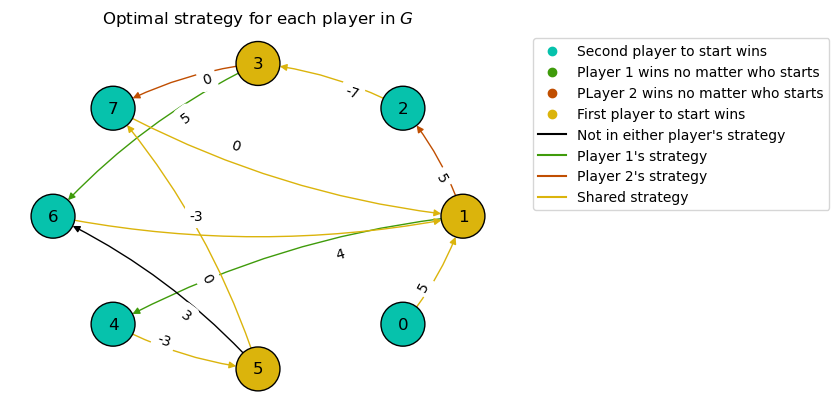
\includegraphics[width= \textwidth]{Figures/OptimalPlayNetworkx.png}
	\caption{Generated visualisation for a Mean Payoff Game with the optimal strategies}
\end{figure}
\FloatBarrier
\subsubsection{games}
This module defines the core functionalities related to mean payoff games.
\newline It also defines the methods to read/write Mean Payoff Graphs. It uses the weighted edgelist format, and supports compression.  
\begin{figure}[H]
	\centering
	\begin{tikzpicture}
		\small
		\begin{package} {networkx}
			\begin{class}{DiGraph}{0,2.5cm}
			\attribute{\dots}
			\operation{\dots}
			\end{class}
		\end{package}
		\begin{package}{ games }
			\begin{class}[text width=12cm]{MeanPayoffGraph}{0,0}
				\inherit{DiGraph}
				\attribute {+ weights\_matrix: Matrix}
				\attribute {+ adjacency\_matrix: Matrix}
				\attribute {+ tensor\_representation: Tensor[3]}
				\operation{+ closure() : MeanPayoffGraph}
				\operation{+ dual() : MeanPayoffGraph}
				\operation {+ as\_bipartite() : MeanPayoffGraph}
				\operation {+ as\_min\_max\_system() : MinMaxSystem}
			\end{class}
			
			\begin{interface}[text width=8.5cm]{Strategy}{0,-5cm}
				\operation{+ \_\_init\_\_(G : MeanPayoffGraph, player : bool)}
				\operation[0]{+ call(vertex : int) : int}
			\end{interface}
			
			\begin{class}[text width=3.5cm]{PositionalStrategy}{-2cm,-8cm}
				\inherit{Strategy}
				\operation[0]{+ call(vertex)}
			\end{class}
			
			\begin{class}[text width=3.5cm]{GreedyStrategy}{-6cm,-8cm}
								\inherit{Strategy}
				\operation[0]{+ call(vertex)}
			\end{class}
			\begin{class}[text width=3.5cm]{EpsGreedyStrategy}{2cm,-8cm}
								\inherit{Strategy}
				\operation[0]{+ call(vertex)}
			\end{class}
			
			\begin{class}[text width=3.5cm]{FractionalStrategy}{6cm,-8cm}
								\inherit{Strategy}
				\operation[0]{+ call(vertex)}
			\end{class}
			
			\begin{class}[text width= 12cm]{Functions}{0,-10cm}
				\operation {@ winning\_everywhere() : bool}
				\operation {@ winning\_somewhere() : bool}
				\operation{@ mpg\_from\_digraph(G : nx.Digraph) : MeanPayoffGraph}
				\operation{@ optimal\_strategy\_pair(G : MeanPayoffGraph) : Tuple[Strategy,Strategy]}
				\operation{@ counter\_strategy(G : MeanPayoffGraph, psi: PositionalStrategy, source : int, player : bool) : Strategy}
				\operation{@ mean\_payoff(G: MeanPayoffGraph, source: int, psi1 : PositionalStrategy, psi2 : PositionalStrategy, turn : bool) : float}
				\operation{@ mean\_payoffs(G: MeanPayoffGraph, psi1 : PositionalStrategy, psi2 : PositionalStrategy) : Matrix}
				\operation{@ winner(G: MeanPayoffGraph, source: int, psi1 : PositionalStrategy, psi2 : PositionalStrategy, turn : bool) : bool}
				\operation{@ winners(G: MeanPayoffGraph, psi1 : PositionalStrategy, psi2 : PositionalStrategy) : Matrix}
			\end{class}
		
		\end{package}
	\end{tikzpicture}
	\caption{\textbf{games} module}
\end{figure}
\FloatBarrier
\subsubsection{ml}
This module defines the required layers, blocks, and model architectures to do machine learning on Mean Payoff Games. This is detailed in chapter \ref{section:ModelDesign}.
\subsubsection{gnn}
This module defines the basic functionalities of graph neural networks \cite{GNN} that are required for our models.

\subsubsection{rl}
This module defines the required functions to do reinforcement learning on Mean Payoff Games\footnote{The current version of this module only supports Mean Payoff Games where at least one player has a fixed strategy.}.

\subsubsection{sp}
This module defines a basic AlphaZero based agent to learn the game.
\subsubsection{wrapper}
This module contains a binding to the C++ implementation of time-critical methods for mean payoff games.
\newline We will give details about this wrapper in the next section.
\subsection{mpgcpp}
This library contains the 
\begin{figure}[H]
	\centering
	\begin{tikzpicture}
		
		\begin{package}{ mpg }
			\begin{class}[text width=3cm]{csp}{0,0}
			\end{class}
			
			\begin{class}[text width=3cm]{games}{4,0}			
			\end{class}
			
			\begin{class}[text width=3cm]{mpgio}{8,0}
			\end{class}
		\end{package}
	\end{tikzpicture}
	\caption{\textbf{mpgcpp} library}
\end{figure}
\subsubsection{csp}
This module contains the constraint satisfaction methods used to solve Mean Payoff Games. 
\subsubsection{games}
This module defines the core functionalities related to mean payoff games.
\begin{figure}[H]
	\centering
	\begin{tikzpicture}
		\small
		\begin{package}{games}
			\begin{abstractclass}[text width=6cm]{MeanPayoffGraphBase}{0,5.5cm}
			\attribute{edges}
			\attribute{dual\_graph}
			\operation[0]{\# add\_edge\_impl(source, target, weight)}
			\operation[0]{\# set\_dual(dual)}
			\operation[0]{+ get\_weight(src, dest)}
			\operation{+ get\_weights()}
			\operation{+ count\_nodes() : int}
			\operation{+ get\_edges() : Edges}
			\end{abstractclass}
			\begin{class}[text width=3.5cm]{VectorMPG}{-6cm,4cm}
				\inherit{MeanPayoffGraphBase}
			\end{class}
			
			\begin{class}[text width=3.5cm]{MatrixMPG}{-6cm,0}
				\inherit{MeanPayoffGraphBase}
			\end{class}
			
			\begin{class}[text width=3.5cm]{HashMapMPG}{6cm,4cm}
				\inherit{MeanPayoffGraphBase}
			\end{class}
			
			\begin{class}[text width=3.5cm]{TreeMapMPG}{6cm,0}
				\inherit{MeanPayoffGraphBase}
			\end{class}
			
			\begin{class}[text width=3.5cm]{DualMPG}{0cm,0cm}
				\inherit{MeanPayoffGraphBase}
			\end{class}
			
			
			\draw[umlcd style,-diamond,fill opacity=100] (DualMPG) to [bend right=12]  (MeanPayoffGraphBase); 
			%\draw[umlcd style,triangle,fill opacity=100] (DualMPG) to [bend right=-12]  (MeanPayoffGraphBase); 
		
			
			\begin{interface}[text width=7.5cm]{Strategy}{0,-2cm}
				\operation{+ \_\_init\_\_(G : MeanPayoffGraph, player : bool)}
				\operation[0]{+ call(vertex : int) : int}
			\end{interface}
			
			\begin{class}[text width=3.5cm]{PositionalStrategy}{-6cm,-5cm}
				\inherit{Strategy}
				\operation[0]{+ call(vertex)}
			\end{class}
			
			\begin{class}[text width=3.5cm]{GreedyStrategy}{-2cm,-5cm}
				\inherit{Strategy}
				\operation[0]{+ call(vertex)}
			\end{class}
			\begin{class}[text width=3.5cm]{EpsGreedyStrategy}{2cm,-5cm}
				\inherit{Strategy}
				\operation[0]{+ call(vertex)}
			\end{class}
			
			\begin{class}[text width=3.5cm]{FractionalStrategy}{6cm,-5cm}
				\inherit{Strategy}
				\operation[0]{+ call(vertex)}
			\end{class}
			
			\begin{class}[text width= 12cm]{Functions}{0,-7cm}
				\operation {@ winning\_everywhere() : bool}
				\operation {@ winning\_somewhere() : bool}
				\operation{@ mpg\_from\_digraph(G : nx.Digraph) : MeanPayoffGraph}
				\operation{@ optimal\_strategy\_pair(G : MeanPayoffGraph) : Tuple[Strategy,Strategy]}
				\operation{@ counter\_strategy(G : MeanPayoffGraph, psi: PositionalStrategy, source : int, player : bool) : Strategy}
				\operation{@ mean\_payoff(G: MeanPayoffGraph, source: int, psi1 : PositionalStrategy, psi2 : PositionalStrategy, turn : bool) : float}
				\operation{@ mean\_payoffs(G: MeanPayoffGraph, psi1 : PositionalStrategy, psi2 : PositionalStrategy) : Matrix}
				\operation{@ winner(G: MeanPayoffGraph, source: int, psi1 : PositionalStrategy, psi2 : PositionalStrategy, turn : bool) : bool}
				\operation{@ winners(G: MeanPayoffGraph, psi1 : PositionalStrategy, psi2 : PositionalStrategy) : Matrix}
			\end{class}
			
		\end{package}
	\end{tikzpicture}
	\caption{\textbf{games} module}
\end{figure}

\subsubsection{mpgio}
Unlike \textbf{mpg}, which has support for mean payoff graph I/O from files via \textbf{NetworkX}. In the C++ library, we have to implement this functionalities from scratch. We used standard I/O utilities with \textbf{boost} to interact with compressed streams conforming to the format used by \textbf{mpg}.
\subsection{Environment}
\subsection{Testing}
\subsection{Structure}
